\begin{figure}[htbp]
\centering
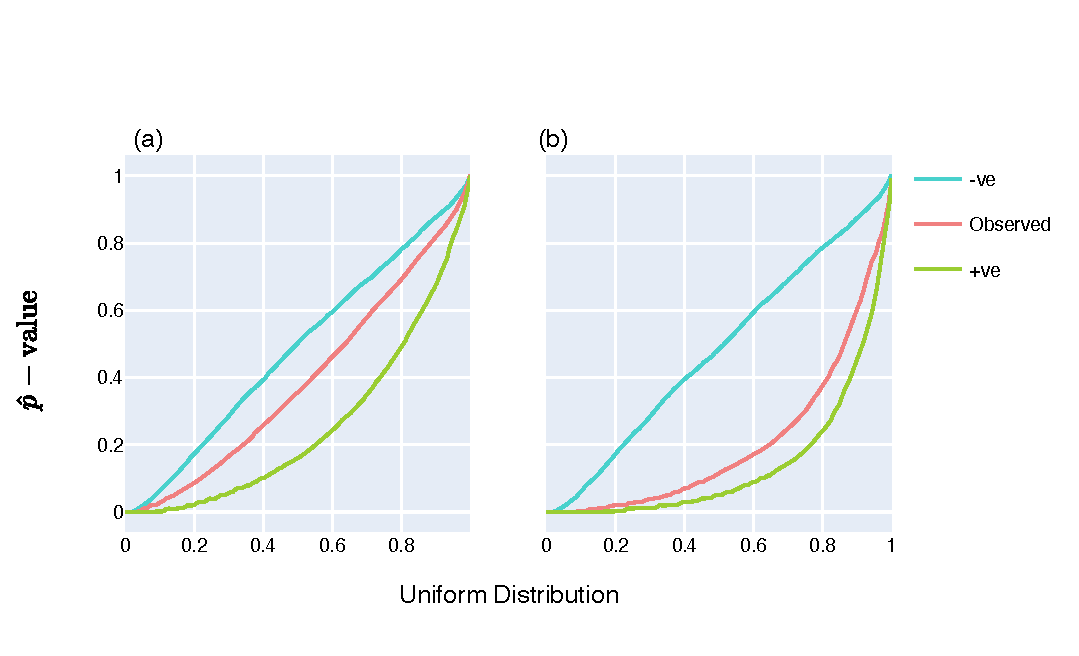
\includegraphics[width=	\textwidth]{figures/plots/drosophila/LRT-QQ.pdf}
\caption[There is a larger proportion of genes in disequilibrium in \textit{D. melanogaster} than in \textit{D. simulans}]{\textbf{There is a larger proportion of genes in disequilibrium in \textit{D. melanogaster} than in \textit{D. simulans}.} The Quantile-Quantile plots compare the distribution of $\hat p-$values to the uniform distribution. The alignments of both plots are from the Drosophila data set with \textbf{(a)}, \textit{D. simulans} modelled as the foreground edge and \textbf{(b)}, \textit{D. melanogaster} modelled as the foreground edge. Each data set contained $\sim 5900$ alignments of \textit{D. melanogaster}, \textit{D. simulans} and \textit{D. yakubra}. }
\label{fig:drosophila_lrt_qq}
\end{figure}
